\clearpage %&latex
\documentclass[a4paper]{article}

\frenchspacing

\usepackage[cp1250]{inputenc}
\usepackage[czech]{babel}

\usepackage{a4wide}
\usepackage{amsmath, amsthm, amssymb, amsfonts}
\usepackage[mathcal]{eucal}
\usepackage{graphicx}
\usepackage{url}
\usepackage{color}
\usepackage{wrapfig}
\usepackage{capt-of}
\usepackage{float}



% sirka a vyska textu nastavena jako papir, vsechny okraje vynulovany a pridano 20pt na kazdou stranu
% horizontalni rozmery
\setlength{\textwidth}{\paperwidth}
\addtolength{\textwidth}{-40pt}
\addtolength{\hoffset}{-1in}
\addtolength{\hoffset}{20pt}
\setlength{\oddsidemargin}{0in}
\setlength{\marginparsep}{0in}
% vertikalni rozmery
\setlength{\textheight}{\paperheight}
\addtolength{\textheight}{-60pt}
\addtolength{\voffset}{-1in}
\addtolength{\voffset}{20pt}
\setlength{\topmargin}{0in}
\setlength{\headheight}{0in}
\setlength{\headsep}{0in}


%Obrazek na miste
%pouziti
%%\obrazeknahore{adresa}{popisek}{label}
\long\def\obrazeknahore#1#2#3 {

\begin{figure}[t]
    \centering
    \includegraphics[width=0.8\textwidth]{#1}
    
    \caption{#2}
    \label{#3}
    
\end{figure}

}


%==========================================
%PEKELNA MAKRA NA ZAROVNANI OBRAZKU DOPRAVA

\makeatletter


%tohle je makro, ktere mi dovoluje obtekani i u kratkych environmentu
%ABSOLUTNE nechapu, jak to funguje, ale funguje to
%viz http://tex.stackexchange.com/questions/26078/ 
\def\odrovnej{\@@par
\ifnum\@@parshape=\z@ \let\WF@pspars\@empty \fi % reset `parshape'
\global\advance\c@WF@wrappedlines-\prevgraf \prevgraf\z@
\ifnum\c@WF@wrappedlines<\tw@ \WF@finale \fi}

\makeatother



%---
%makro, co da obrazek doprava a ostatni text ho obteka
%(bez toho predchazejiciho makra to ale poradne nebeha)
%pouziti:
%\obrazekvpravo{adresa}{popisek}{label}{procento sirky}
\long\def\obrazekvpravo#1#2#3#4{

\setlength\intextsep{-20pt}

    \begin{wrapfigure}{r}{#4\textwidth}
      \begin{center}
          \vspace{-10pt}
          
        \includegraphics[width=#4\textwidth]{#1}
        \vspace{-10pt}
        
      \end{center}
      
      \caption{#2}
      \label{#3}
      
      
    \end{wrapfigure}

\setlength\intextsep{0pt}

    
}




%---
%makro pro pripady, kdy wrapfigure neco mrsi
%je to docela pekelne
%je nutne mu dat jak text vpravo, tak text vlevo
%a nevim, jestli bude 100% fungovat, ale doufam, ze jo

%pouziti:
%\obrazekvpravominipage{adresa}{popisek}{label}{procento sirky}{1 - procento sirky}{text vlevo}
\long\def\obrazekvpravominipage#1#2#3#4#5#6{

\noindent\begin{minipage}{#5\linewidth}
\vspace{0pt}
#6
\end{minipage}
\hspace{0.5cm}
\noindent\begin{minipage}{#4\linewidth}
\vspace{0pt}
\centering
\includegraphics[width=0.9\textwidth]{#1}
\captionof{figure}{#2}
\label{#3}
\end{minipage}

}

%KONEC PEKELNYCH MAKER
%=====================

% makra pro poznamku u vyrokove a predikatove logiky
\def\vl{ -- ve v�rokov� logice}
\def\pl{ -- v predik�tov� logice}


%Vacsina prostredi je dvojjazicne. V pripade, ze znenie napr pozorovania je pisane po slovensky, malo by byt po slovensky aj oznacenie.

\newenvironment{pozadavky}{\pagebreak[2]\noindent\textbf{Po�adavky}\par\noindent\leftskip 10pt}{\odrovnej\par\bigskip}
\newenvironment{poziadavky}{\pagebreak[2]\noindent\textbf{Po�iadavky}\par\noindent\leftskip 10pt}{\odrovnej\par\bigskip}


\newenvironment{definiceSkull}{\pagebreak[2]\noindent\textbf{$\bigstar$ Definice}\par\noindent\leftskip 10pt}{\odrovnej\par\bigskip}
\newenvironment{definiceNSkull}[1]{\pagebreak[2]\noindent\textbf{$\bigstar$ Definice~}\emph{(#1)}\par\noindent\leftskip 10pt}{\odrovnej\par\bigskip}

\newenvironment{definice}{\pagebreak[2]\noindent\textbf{Definice}\par\noindent\leftskip 10pt}{\odrovnej\par\bigskip}
\newenvironment{definiceN}[1]{\pagebreak[2]\noindent\textbf{Definice~}\emph{(#1)}\par\noindent\leftskip 10pt}{\odrovnej\par\bigskip}
\newenvironment{definicia}{\pagebreak[2]\noindent\textbf{Defin�cia}\par \noindent\leftskip 10pt}{\odrovnej\par\bigskip}
\newenvironment{definiciaN}[1]{\pagebreak[2]\noindent\textbf{Defin�cia~}\emph{(#1)}\par\noindent\leftskip 10pt}{\odrovnej\par\bigskip}

\newenvironment{vetaSkull}{\pagebreak[2]\noindent\textbf{$\bigstar$ V�ta}\par\noindent\leftskip 10pt}{\odrovnej\par\bigskip}
\newenvironment{vetaNSkull}[1]{\pagebreak[2]\noindent\textbf{$\bigstar$ V�ta~}\emph{(#1)}\par\noindent\leftskip 10pt}{\odrovnej\par\bigskip}

\newenvironment{pozorovani}{\pagebreak[2]\noindent\textbf{Pozorov�n�}\par\noindent\leftskip 10pt}{\odrovnej\par\bigskip}
\newenvironment{pozorovanie}{\pagebreak[2]\noindent\textbf{Pozorovanie}\par\noindent\leftskip 10pt}{\odrovnej\par\bigskip}
\newenvironment{poznamka}{\pagebreak[2]\noindent\textbf{Pozn�mka}\par\noindent\leftskip 10pt}{\odrovnej\par\bigskip}
\newenvironment{poznamkaN}[1]{\pagebreak[2]\noindent\textbf{Pozn�mka~}\emph{(#1)}\par\noindent\leftskip 10pt}{\odrovnej\par\bigskip}
\newenvironment{lemma}{\pagebreak[2]\noindent\textbf{Lemma}\par\noindent\leftskip 10pt}{\odrovnej\par\bigskip}
\newenvironment{lemmaN}[1]{\pagebreak[2]\noindent\textbf{Lemma~}\emph{(#1)}\par\noindent\leftskip 10pt}{\odrovnej\par\bigskip}
\newenvironment{veta}{\pagebreak[2]\noindent\textbf{V�ta}\par\noindent\leftskip 10pt}{\odrovnej\par\bigskip}
\newenvironment{vetaN}[1]{\pagebreak[2]\noindent\textbf{V�ta~}\emph{(#1)}\par\noindent\leftskip 10pt}{\odrovnej\par\bigskip}
\newenvironment{vetaSK}{\pagebreak[2]\noindent\textbf{Veta}\par\noindent\leftskip 10pt}{\odrovnej\par\bigskip}
\newenvironment{vetaSKN}[1]{\pagebreak[2]\noindent\textbf{Veta~}\emph{(#1)}\par\noindent\leftskip 10pt}{\odrovnej\par\bigskip}

\newenvironment{dusledek}{\pagebreak[2]\noindent\textbf{D�sledek}\par\noindent\leftskip 10pt}{\odrovnej\par\bigskip}
\newenvironment{dosledok}{\pagebreak[2]\noindent\textbf{D�sledok}\par\noindent\leftskip 10pt}{\odrovnej\par\bigskip}

\newenvironment{dokaz}{\pagebreak[2]\noindent\leftskip 10pt\textbf{D�kaz}\par\noindent\leftskip 10pt}{\odrovnej\par\bigskip}
\newenvironment{dukaz}{\pagebreak[2]\noindent\leftskip 10pt\textbf{D�kaz}\par\noindent\leftskip 10pt}{\odrovnej\par\bigskip}

\newenvironment{ideadukazu}{\pagebreak[2]\noindent\leftskip 10pt\textbf{Idea d�kazu}\par\noindent\leftskip 10pt}{\odrovnej\par\bigskip}


\newenvironment{priklad}{\pagebreak[2]\noindent\textbf{P��klad}\par\noindent\leftskip 10pt}{\odrovnej\par\bigskip}
\newenvironment{prikladN}[1]{\pagebreak[2]\noindent\textbf{P��klad~}\emph{(#1)}\par\noindent\leftskip 10pt}{\odrovnej\par\bigskip}

\newenvironment{prikladSK}{\pagebreak[2]\noindent\textbf{Pr�klad}\par\noindent\leftskip 10pt}{\odrovnej\par\bigskip}
\newenvironment{priklady}{\pagebreak[2]\noindent\textbf{P��klady}\par\noindent\leftskip 10pt}{\odrovnej\par\bigskip}
\newenvironment{prikladySK}{\pagebreak[2]\noindent\textbf{Pr�klady}\par\noindent\leftskip 10pt}{\odrovnej\par\bigskip}

\newenvironment{algoritmusN}[1]{\pagebreak[2]\noindent\textbf{Algoritmus~}\emph{(#1)}\par\noindent\leftskip 10pt}{\odrovnej\par\bigskip}
%obecne prostredie, ktore ma vyuzitie pri specialnych odstavcoch ako (uloha, algoritmus...) aby nevzniklo dalsich x prostredi
\newenvironment{obecne}[1]{\pagebreak[2]\noindent\textbf{#1}\par\noindent\leftskip 10pt}{\odrovnej\par\bigskip}

\newenvironment{report}{\pagebreak[2]\noindent\textbf{Report}\em\par\noindent\leftskip 10pt}{\par\bigskip}

%\newenvironment{reportN}[1]{\pagebreak[2]\noindent\textbf{Report~}\emph{(#1)}\emph\par\noindent\leftskip 10pt}{\odrovnej\par\bigskip}
\newenvironment{reportN}[1]{\pagebreak[2]\noindent\textbf{Report~}\emph{(#1)}\em\par\noindent\leftskip 10pt}{\odrovnej\par\bigskip}

\newenvironment{penumerate}{
\begin{enumerate}
  \setlength{\itemsep}{1pt}
  \setlength{\parskip}{0pt}
  \setlength{\parsep}{0pt}
  %\setlength{\topsep}{200pt}
  \setlength{\partopsep}{200pt}
}{\end{enumerate}}

\def\pismenka{\numberedlistdepth=2} %pouzit, ked clovek chce opismenkovany zoznam...

\newenvironment{pitemize}{
\begin{itemize}
  \setlength{\itemsep}{1pt}
  \setlength{\parskip}{0pt}
  \setlength{\parsep}{0pt}
}{\end{itemize}}

%\definecolor{gris}{gray}{0.95}
\newcommand{\ramcek}[2]{\begin{center}\fcolorbox{white}{gris}{\parbox{#1}{#2}}\end{center}\par}
 \clearpage
\title{\LARGE Učební texty k státní bakalářské zkoušce \\ Obecná informatika \\ Programovací jazyky}
\begin{document}
\maketitle
\newpage
\setcounter{section}{5}
\section{Programovací jazyky}
\begin{pozadavky}
\begin{pitemize}
\item Principy implementace procedurálních programovacích jazyků, oddělený překlad, sestavení.
\item Objektově orientované programování.
\item Neprocedurální programování, logické programování.
\item Generické programování.
\end{pitemize}
\end{pozadavky}
\subsection{Principy implementace procedur�ln�ch a objektov� orientovan�ch programovac�ch jazyk�, odd�len� p�eklad, sestaven�}

Principy implementace proceduralnich programovacich jazyku je v zasade jednoducha vec. Je treba vedet, jak funguji zakladni veci uvnitr. Ze program ma ctyri kusy pameti (code, data, stack a heap) a co ktera dela. Jak probiha volani procedur, kam se pri nem co schova. Jak funguje rekurze, kam se ukladaji lokalni promenne a kam globalni, ... atd. 



\subsubsection*{Strukturovan� programov�n�}

Po��ta�ov� program je n�jak�m zp�sobem zaznamenan� postup po��ta�ov�ch operac�, kter� speci�ln�m zp�sobem popisuje praktickou realizaci zadan� �lohy (tedy algoritmus v�po�tu). Program z \emph{procedur�ln�ho} �hlu pohledu je vlastn� p�esn� specifikace v�ech krok�, kter� mus� po��ta� vykonat, aby do�el k c�li, a jejich po�ad�. Pro ur�ov�n� po�ad� krok� se pou��vaj� z�kladn� operace \emph{��zen� toku} -- skoky, podm�nky, cykly apod.

Jedn�m z d�le�it�ch koncept� procedur�ln�ho programov�n� je \emph{strukturovan� programov�n�} -- jeho idea je zalo�ena na rod�len� programu na \emph{procedury} (rutiny, podrutiny, metody, funkce), kter� samy obsahuj� v��et v�po�etn�ch krok� k vykon�n�, mohou b�t ale spou�t�ny opakovan� a z libovoln�ho m�sta v programu. Jejich v�hodou je mnohem n�zorn�j�� pohled na strukturu programu a snaz�� udr�ov�n� k�du, ne� v p��pad� pou�it� jen nejjednodu���ho ��zen� toku (tedy hlavn� skok�, kter� by se ve strukturovan�m programov�n� spr�vn� pou��vat nem�ly).



\subsubsection*{Datov� a~��d�c� struktury vy���ch programovac�ch jazyk� a~jejich implementace}

\begin{obecne}{��zen� toku}
V informatice se \emph{tokem ��zen�} rozum� po�ad� ve kter�m se prov�d�j� jednotliv� p��kazy programu. V imperativn�ch (=procedur�ln�ch) programovac�ch jazyc�ch se \emph{p��kazy pro ��zen� toku} rozum� p��kazy, kter� dok�ou zm�nit po�ad� prov�d�n� p��kaz� na jin� ne� p�irozen� (to v jak�m jsou zaps�ny). N�kter� funkcion�ln� jazyky tak� obsahuj� takov� p��kazy (kter� ji� nepat�� do funkcion�ln�ho programov�n�), ale potom u� se jim v�t�inou ne��k� p��kazy pro ��zen� toku.
\\\\
Druhy p��kaz� pro ��zen� toku se mezi jazyky li��, ale p�ibli�n� mohou b�t rozd�leny do n�sleduj�c�ch kategori�.
\begin{pitemize}
\item Pokra�ov�n� na jin�m m�st� programu (skok).
\item Vykon�n� skupiny p��kaz� pouze pokud je spln�na ur�it� podm�nka (if-then-else)
\item Nevykon�n� skupiny p��kaz� nebo jejich opakov�n� do t� doby ne� je spln�na ur�it� podm�nka (smy�ka/cyklus). Cykly mohou b�t s podm�nkou na za��tku, na konci, uprost�ed, nekone�n�, s dan�m po�tem opakov�n�.
\item Vykon�n� skupiny p��kaz�, kter� se nach�zej� na jin�m m�st� k�d�, a n�sledn� (voliteln�) vr�cen� ��zen� toku zp�t (subroutines, coroutines, and continuations).
\item Zastaven�/ukon�en� programu.
\end{pitemize}

\emph{P�eru�en� a sign�ly} jsou n�zko�rov�ov� mechanizmus, kter� m��e zm�nit tok ��zen� podobn� jako se to d�l� u podprogram�, ale v�t�inou je vyvol�n vn�j�� ud�lost� a nen� tedy pou�it ve smyslu ��zen� toku programu, jak bylo pops�no.
\end{obecne}

\begin{obecne}{V�jimky}
V�jimky jsou speci�ln�m p��kazem ��zen� toku, vyskytuj�c�m se v n�kter�ch vy���ch programovac�ch jazyc�ch. Z�kladn� my�lenkou je, �e program m��e na n�jak�m m�st� vyhodit v�jimku (p��kaz \texttt{throw}), co� zp�sob�, �e prov�d�n� programu se zastav� a bu� pokra�uje tam, kde je v�jimka \uv{o�et�ena} (tzv. \texttt{catch} blok), nebo pokud takov� m�sto nen� nalezeno, program skon�� s chybou. B�hem hled�n� m�sta o�et�en� je datov� hodnota v�jimky ulo�ena stranou a pak m��e b�t pou�ita.

P�i hled�n� m�sta o�et�en� v�jimky (\texttt{try}-bloku, n�sledovan�ho catch-blokem se spr�vn�m datov�m typem v�jimky) se postupuje zp�t po z�sobn�ku vol�n� funkc�, tato technika se naz�v� \uv{stack unwinding} (odv�jen� z�sobn�ku). V n�kter�ch jazyc�ch (Java) lze definovat i akci, kter� se provede v ka�d�m p��pad�, i pokud nastane v�jimka, je�t� p�ed odv�jen�m z�sobn�ku -- \texttt{finally} blok.
\end{obecne}

\begin{obecne}{Volac� konvence}
P�i vol�n� procedur a funkc� je nejd�le�it�j�� z�sobn�k. Ukl�d� se na n�j
\begin{pitemize}
    \item kam se vr�tit po vol�n�
    \item argumenty funkce (v p�ekladem definovan�m po�ad� -- nutn� m�t ve v�ech modulech stejn�; v�t�inou se li�� v z�vislosti na programovac�m jazyku)
    \item n�vratov� hodnota funkce
    \item ukazatel na s�manticky nad�azenou funkci (Pascal)
\end{pitemize}
Dohromady v�em t�mto dat�m se n�kdy ��k� \emph{aktiva�n� z�znam} procedury. Po skon�en� funkce je nutn� z�sobn�k op�t uklidit (vymazat zbyte�n� ulo�en� data, v�t�inou jen z�st�v� n�vratov� hodnota) a kter� ��st programu to d�l� (volan� nebo volaj�c� procedura), z�vis� op�t na p�eklada�i a konvenci jazyka.

\medskip\noindent
Volac� konvence dvou nejtypi�t�j��ch jazyk�:
\begin{pitemize}
\item \emph{Pascal} \\ ukl�z� volan� funkce, argumenty se ukl�daj� na z�sobn�k zleva doprava (nejlevej�� nejd��v, tj. nejhloub�ji)
\item \emph{C} \\ ukl�z� funkce volaj�c�, argumenty se ukl�daj� zprava doleva (tj. nejlev�j�� je na vrcholu z�sobn�ku. Je to kv�li funkc�m s prom�nn�m po�tem parametr�. Volan� funkce mus� podle prvn�ho argumentu poznat, jak� je skute�n� po�et argument�. Kdyby byl prvn� argument n�kde hluboko v~z�sobn�ku, tak v� prd.)
\end{pitemize}
\end{obecne}

\begin{obecne}{Vol�n� funkc� a procedur z pohledu procesoru}
\begin{penumerate}
    \item ulo�en� vstupn�ch parametr� pro funkci
    \item p�ed�n� ��zen� do k�du funkce - \uv{skok}
    \item z�sk�n� prost�edk� pro vykon�n� funkce
    \item proveden� po�adovan� funkce
    \item ulo�en� v�sledk� pro volaj�c�ho
    \item n�vrat do m�sta vol�n�
\end{penumerate}
M�me registry pro data (vstupn� parametry a n�vratovou hodnotu) a registr pro n�vratovou hodnotu, kam se ulo�� adresa instrukce n�sleduj�c� po instrukci vol�n� (neboli hodnota Program Counteru PC + 4).\\
V p��pad� rekurzivn�ho vol�n� nebo v�t��ho po�tu parametr� mus�me registry dostat na z�sobn�k v pam�ti (ten roste sm�rem k ni���m adres�m, tj. ��m v�t�� z�sobn�k, t�m ni��� hodnota stack pointeru SP).
\end{obecne}


\subsubsection*{Organizace pam�ti}

Pam� procesu (spu�t�n�ho programu) lze rozd�lit do n�kolika ��st�:
\begin{pitemize}
\item \emph{k�d programu (k�dov� segment)} \\
vytvo�en p�i p�ekladu, sou��st spustiteln�ho souboru, nem�nn� a m� pevnou d�lku; obvykle b�v� chr�n�n proti z�pisu
\item \emph{statick� data (datov� segment)} \\
data programu, jejich� velikost je zn�ma ji� p�i p�ekladu a jejich� pozice se b�hem programu nem�n� (je p�ipraven kompil�torem a jeho form�t je takt� zadr�tovan� ve spustiteln�m souboru, u inicializovan�ch statick�ch dat je tam cel� ulo�en�); v jazyce C jde o glob�ln� prom�nn� a lok�ln� data deklarovan� jako \texttt{static}, konstanty
\item \emph{halda (heap segment)} \\
vytv��en startovac�m modulem (C Runtime library), ukl�daj� se sem dynamicky vznikaj�c� objekty (\texttt{malloc, new}) -- neinicializovan� data, i seznam voln�ho m�sta
\item \emph{voln� pam�} \\
postupn� j� zapl�uje z jedn� strany z�sobn�k a z druh� halda
\item \emph{z�sobn�k (stack segment)} \\
informace o vol�n� procedur (\uv{aktiva�n� z�znamy}) --- n�vratov� adresy, parametry a n�vratov� hodnoty (nejsou-li p�ed�v�ny v registrech), n�kter� jazyky (Pascal, C) pou��vaj� i pro �schovu lok�ln�ch dat. Typicky roste z�sobn�k proti hald� (od \uv{konce} pam�ti k ni���m adres�m).
\end{pitemize}


\begin{e}{Pozn�mka}{0}{Vno�en� funkce}
V Pascalu mohou b�t funkce definovan� uvnit� jin� funkce. Ta vnit�n� pot�ebuje p�istupovat k~prom�nn�m t� vn�j��. Prom�nn� jsou sice na z�sobn�ku, ale pouh� odkaz na volaj�c� funkci nesta��, proto�e se vno�en� funkce m��e volat rekurzivn�. Proto je na z�sobn�ku ukazatel na funkci s�manticky nad�azenou.
\end{e}

\begin{obecne}{Alokace m�sta pro r�zn� typy prom�nn�ch}
\begin{pitemize}
    \item Dynamicky alokovan� prom�nn� (p�es pointer) se alokuj� na hald�. Opakovanou alokac� a~dealokac� pam�ov�ch blok� r�zn� velikosti vznikaj� v~hald� \uv{d�ry} (st��dav� �seky voln�ho a naalokovan�ho m�sta). Existuje n�kolik strategi� pro vyhled�n� voln�ho bloku po�adovan� velikosti (first-fit, next-fit, buddy syst�m) a udr�en� informac� o voln�m m�st�, kter� jsou v�t�inou implementov�ny v knihovn�ch funkc�ch jazyka (C, Pascal).
    \item Lok�ln� prom�nn� se ukl�daj� na z�sobn�k, po skon�en� funkce, kter� p��slu��, jsou zase odstran�ny.
    \item Glob�ln� a~statick� se ukl�daj� do segmentu pro statick� data. Tady se d�ry tvo�it nebudou, proto�e tyhle prom�nn� vznikaj� na za��tku a~zanikaj� na konci programu (tak�e se form�t segmentu nem�n�).
\end{pitemize}
\end{obecne}

\subsubsection*{Odd�len� p�eklad, sestaven�}

\begin{obecne}{Struktura programu}

Program se skl�d� z \emph{modul�}:
\begin{pitemize}
        \item P�ekl�d�ny samostatn� kompil�torem 
        \item Spojov�ny linkerem
\end{pitemize}
Modul z pohledu program�tora
\begin{pitemize}
        \item Soubor s p��ponou .cpp (.c)
\end{pitemize}
Hlavi�kov� soubory
\begin{pitemize}
        \item Soubory s p��ponou .h
        \item Deklaruj� (a n�kdy i definuj�) identifik�tory pou��van� ve v�ce modulech
        \item Vkl�d�ny do modul� direktivou include
        \begin{pitemize}
                \item Direktivu zpracov�v� preprocesor �ist� textov�
                \item Preprocesor je integrov�n v kompil�toru jako prvn� f�ze p�ekladu
        \end{pitemize}
\end{pitemize}
Modul z pohledu kompil�toru
\begin{pitemize}
        \item Samostatn� jednotka p�ekladu
        \item V�sledek pr�ce preprocesoru
\end{pitemize}
\end{obecne}


\begin{obecne}{Odd�len� p�eklad}

\par\begin{center}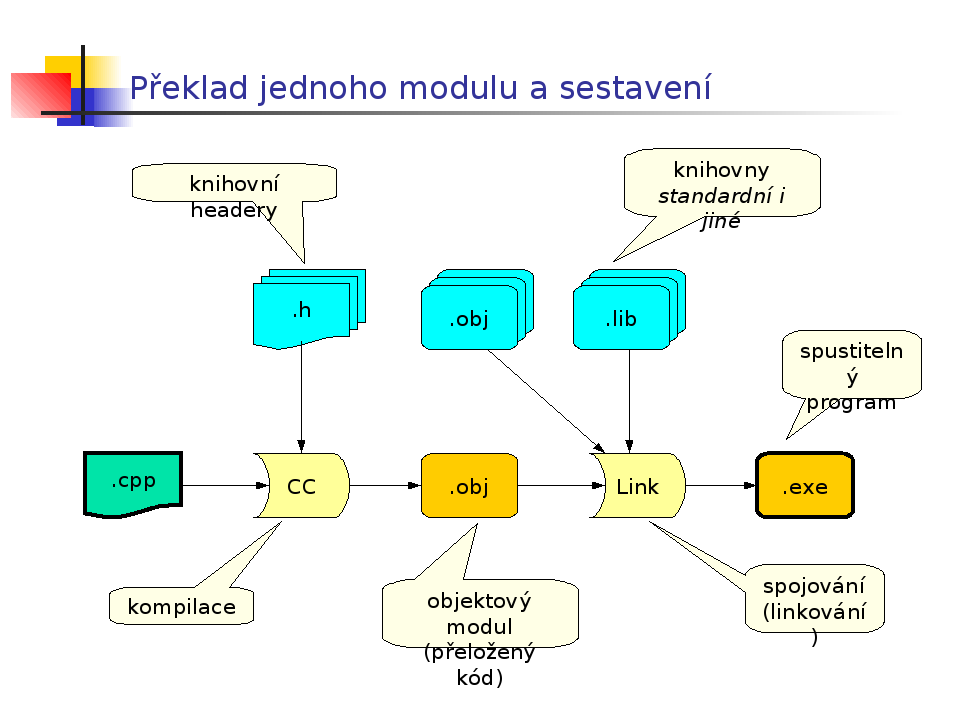
\includegraphics[width=10cm]{informatika/programovanie/obrazky/oddelenypreklad01.png}
\end{center}
\par\begin{center}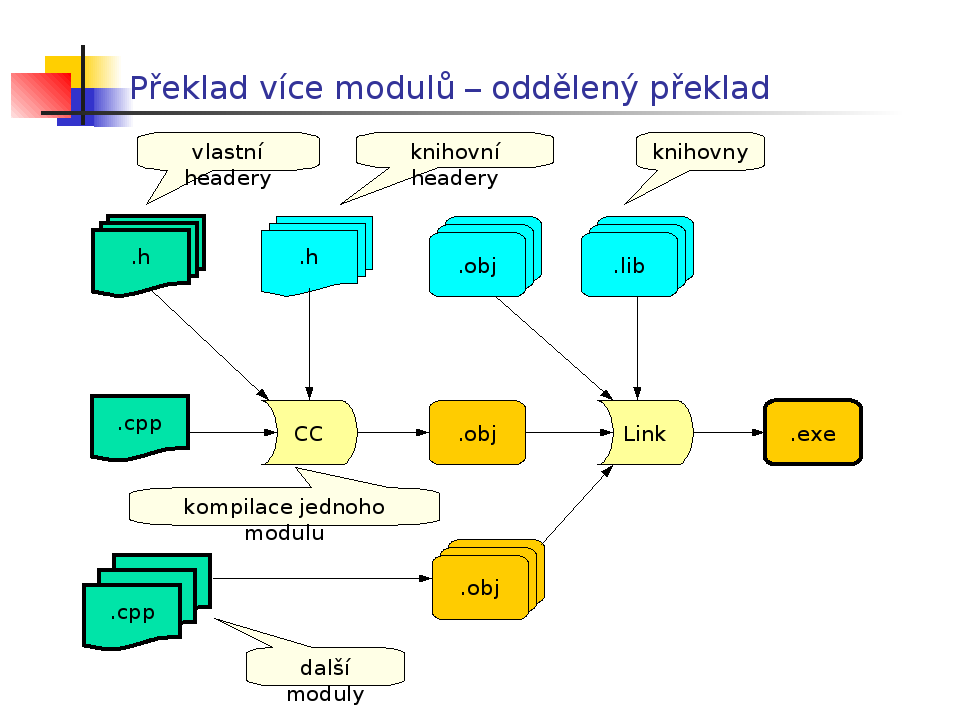
\includegraphics[width=10cm]{informatika/programovanie/obrazky/oddelenypreklad02.png}\end{center}
Smysl odd�len�ho p�ekladu modul� je urychlen� celkov�ho p�ekladu -- nep�ekl�dat to, co se od minula nezm�nilo. Odd�len� p�eklad dnes d�ky automatizaci makefily (viz n�e) a integrovan�mi prost�ed�mi nen� t�m�� pro program�tora vid�t.

...na tomto slide je vhodn� si ujasnit, jak funguje statick� a dynamick�
linkov�n� (jak a kde a kdy se opravuj� adresy objekt� atd...):
\begin{pitemize}
    \item \emph{Statick� linkov�n�} \\ Po odd�len�m p�ekladu jednotliv� object moduly je�t� neobsahuj� p��mo adresy v�ech funkc� a extern�ch identifik�tor�, jen odkazy na n�. Linker se postar� o jejich spojen� dohromady. Je nutn�, aby jm�na byla unik�tn�, tak�e u p�et�en�ch a virtu�ln�ch funkc�, jako je v C++, mus� b� jm�na zpotvo�ena tak, aby ukazovala i t��du, namespace, parametry a jejich typy. To m� na starosti compiler a ��k� se tomu \emph{name mangling}.
    \item \emph{Dynamick� linkov�n�} \\ Nast�v� po vol�n� opera�n�ho syst�mu -- zaveden� dynamick� knihovny do pam�ti. Jsou dv� mo�nosti jeho proveden�, prvn� je pr�v� p�i zav�d�n� knihovny, kdy se odkazy na v�echny funkce (a mezi nimi navz�jem) napln� spr�vn�mi hodnotami (podle b�zov� adresy, na kterou se knihovna do pam�ti nahraje). Druh� mo�nost je pou�it� dvou pointer� p�i vol�n� funkc� z knihovny -- to se vytvo�� tabulka skute�n�ch adres, na kterou se z knihovny ukazuje. Prvn� mo�nost trv� d�le p�i zav�d�n� knihovny, druh� je zase pomalej�� p�i prov�d�n�, ale umo��uje k�d knihovny beze zm�n sd�let v�ce procesy.
\end{pitemize}


\par\begin{center}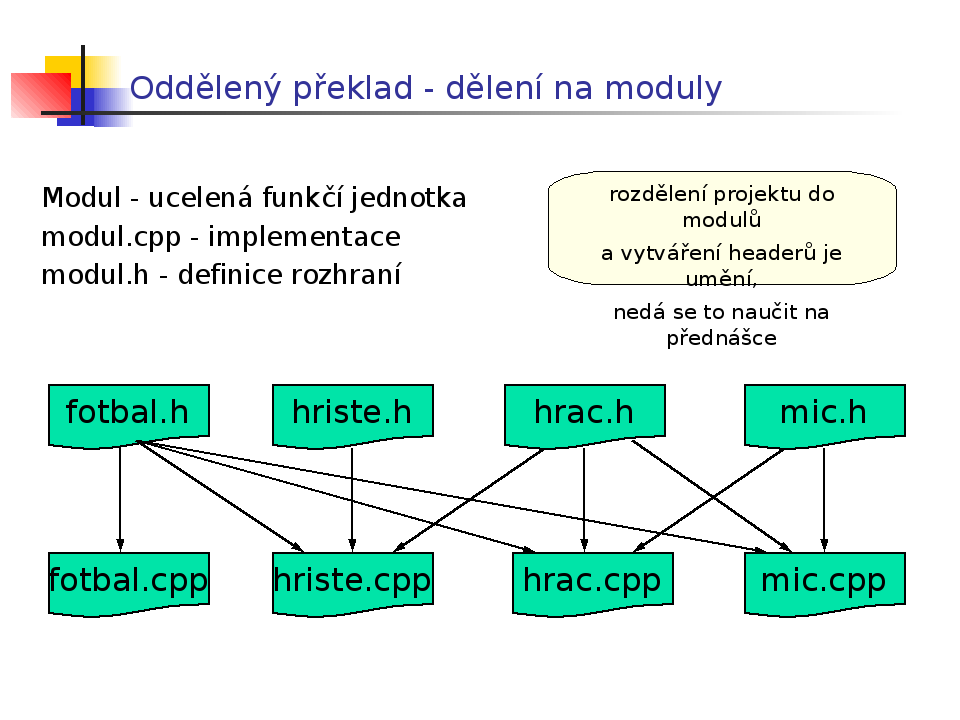
\includegraphics[width=10cm]{informatika/programovanie/obrazky/oddelenypreklad03.png}\end{center}

\emph{Linker} je program, kter� prij�m� jeden alebo v�ce objekt� generovan�ch kompil�torem a slo�� je v jeden spustiteln� program.

Objektov� k�d, nebo objektov� soubor je reprezentace k�du, kter� kompil�tor nebo assembler vytvo�� zpracov�n�m zdrojov�ho k�du. Objektov� soubory obsahuj� kompaktn� k�d, �asto naz�van� \uv{bin�rky} :-) Linker se typicky pou��v� na vytvo�en� spustiteln�ho souboru nebo knihovny spojen�m (slinkov�n�m) objektov�ch soubor�. Z�kladn� �ast� objektov�ho souboru je strojov� k�d (k�d p�imo vykon�van� CPU po��ta�e).
\end{obecne}
\begin{obecne}{Makefile}

Smyslem programu \emph{make} je ��zen� p�ekladu a linkov�n�. Popis z�vislost� jednotliv�ch modul� a hlavi�kov�ch soubor� je definov�n v 1 textov�m souboru -- \emph{Makefile} (tj. kter� soubory je nutn� m�t aktu�ln�/vytvo�en� pro p�eklad kter�ho souboru). Make v�dy po zm�n� souboru p�elo�� jen to, co na n�m z�vis�.
Form�t souboru make:
\begin{verbatim}
targets: files; 
        commands; #comment; line-begin\
        line contd.;
\end{verbatim}
Targets -- c�le �innost� / c�lov� soubory, mo�no definovat vic, p�i spu�t�n� make bez parametr� se bere prvn�; univ. n�stroj (nejen pro p�eklad C/C++). Lze definovat i vlastn� makra (p��kazem \texttt{<n�zev makra> = <string>}) a pak je pou��vat (\texttt{\$\{makro\}}).
\end{obecne}

\newpage\subsection{Objektov� orientovan� programov�n�\footnote{podle zkou�en� Bure�em a T�mou}}  

\begin{obecne}{��el objektov�ho porgramov�n�}
In the 1960s, language design was often based on textbook examples of programs, which were generally small (due to the size of a textbook); however, when programs become very large, the focus changes. In small programs, the most common statement is generally the assignment statement; however, in large programs (over 10,000 lines), the most common statement is typically the procedure-call to a subprogram. Ensuring parameters are correctly passed to the correct subprogram becomes a major issue.

Many small programs can be handled by coding a hierarchy of structures; however, in large programs, the organization is more a network of structures, and insistence on hierarchical structuring for data and procedures can produce cumbersome code with large amounts of "tramp data" to handle various options across the entire program.

Although structuring a program into a hierarchy might help to clarify some times of software, even for some special types of large programs, a small change, such as requesting a user-chosen new option (text font-color) could cause a massive ripple-effect with changing multiple subprograms to propagate the new data into the program's hierarchy. The object-oriented approach is allegedly more flexible, by separating a program into a network of subsystems, with each controlling their own data, algorithms, or devices across the entire program, but only accessible by first specifying named access to the subsystem object-class, not just by accidentally coding a similar global variable name. Rather than relying on a structured-programming hierarchy chart, object-oriented programming needs a call-reference index to trace which subsystems or classes are accessed from other locations.
\end{obecne}


\begin{definiceN}{Objektov� orientovan� programov�n�}
Objektov� orientovan� programov�n� (zkracov�no na OOP, z anglick�ho Object-oriented programming) je metodika v�voje softwaru. D� se na n�j nahl�dnout jako na kolekci spolupracuj�c�ch objekt� -- v protikladu k tradi�n�mu pohledu, kdy se za program pova�uje sled instrukc� pro po��ta�. V OOP je ka�d� objekt schopn� p�ij�mat zpr�vy, zpracov�vat data a pos�lat zpr�vy jin�m objekt�m. Na ka�d� objekt se tak d� nahl�et jako na nez�visl� \uv{mal� stroj} s vlastn� rol� a zodpov�dnost�. Zjednodu�en� �e�eno jde o~dota�en� konceptu \emph{data + algoritmy = program}. Data tvo�� s k�dem, kter� je spravuje, jeden celek.
Je zalo�eno na n�sleduj�c�ch my�lenk�ch, koncepci:
\end{definiceN}
\begin{obecne}{Objekty} Jednotliv� prvky modelovan� reality (jak data, tak souvisej�c� funk�nost) jsou v programu seskupeny do entit, naz�van�ch objekty. Objekty si pamatuj� sv�j stav a navenek poskytuj� operace (p��stupn� jako metody pro vol�n�).
\\\\
\textbf{Implementace objekt�}
Z hlediska jazyka nen� velk� rozd�l mezi slo�en�mi datov�mi typy a t��dami. Deklarace t��dy obsahuje, stejn� jako u slo�en�ho dat. typu, datov� polo�ky. Nav�c ale obsahuje i deklarace funkc� (metod), kter� s nimi pracuj�. N�kter� funkce mohou m�t speci�ln� vlastnosti -- statick�, virtu�ln�, konstruktory, destruktory. Nav�c v�t�ina jazyk� p�id�v� mo�nost ozna�en� kter�chkoliv polo�ek jako ve�ejn� nebo priv�tn�. T��dy mohou n�kdy (C++, Java) obsahovat i vno�en� datov� typy (v��ty, ... ) a dokonce vno�en� t��dy.

Za b�hu je jedna instance t��dy -- objekt reprezentov�na v pam�ti pomoc�:
\begin{pitemize}
    \item datov�ch polo�ek (stejn� jako slo�en� datov� typ),
    \item skryt�ch pomocn�ch polo�ek umo��uj�c�ch funkci virtu�ln�ch metod, v�jimek, RTTI a d�di�nosti (identifikace typu / jeho velikosti apod.)
\end{pitemize}
\end{obecne}

\begin{obecne}{Abstrakce} Program�tor, pota�mo program, kter� vytv���, m��e abstrahovat od n�kter�ch detail� pr�ce jednotliv�ch objekt�. Ka�d� objekt pracuje jako �ern� sk���ka, kter� dok�e prov�d�t ur�en� �innosti a komunikovat s okol�m, ani� by vy�adovala znalost zp�sobu, kter�m vnit�n� pracuje.

\end{obecne}
\begin{obecne}{Zapouzd�en�} Zaru�uje, �e objekt nem��e p��mo p�istupovat k \uv{vnit�nostem} jin�ch objekt�, co� by mohlo v�st k nekonzistenci. Ka�d� objekt navenek zp��stup�uje rozhran�, pomoc� kter�ho (a nijak jinak) se s objektem pracuje.
\\\\
\textbf{Jake ma vyhody OOP proti pouze proceduralnimu programovani} - Zacal jsem zapouzdrenim, kde me vcelku potrapil pure C jazykem jehoz moduly, .h soubory, pouziti staticu, ifdefu a dalsich konstruktu muze slouzit jako slusne zapouzdreni - ukolem bylo rict na konkretnim jazyce co prinasi OOP navic (napr. vetsi granularita oddeleni (Java a viditelnost v Packagi, protected, final...))
\\\\
We use these keywords to specify access levels for member variables, or for member functions (methods).
\begin{pitemize}
    \item \textbf{public} variables, are variables that are visible to all classes.
    \item \textbf{private} variables, are variables that are visible only to the class to which they belong.
    \item \textbf{protected} variables, are variables that are visible only to the class to which they belong, and any subclasses.
\end{pitemize}
\end{obecne}

\begin{obecne}{Skl�d�n�}Objekt m��e vyu��vat slu�eb jin�ch objekt� tak, �e je po��d� o proveden� operace.
\end{obecne}

\begin{obecne}{T��da}
\emph{T��da} definuje abstraktn� vlastnosti n�jak�ho objektu, v�etn� obsa�en�ch dat (atributy, pole (fields) a vlastnosti (properties)) a v�c�, kter� m��e d�lat (chov�n�, metody a schopnosti (features)). Nap��klad t��da \emph{Dog} by obsahovala v�ci spolo�n� pro v�echny psy - nap�. atributy rasa, barva srsti a schopnosti �t�kat. % tady prosim ten jazyk neopravujte, to je tak hezky :)!
 

T��dy poskytuj� v objektov�-orientovan�m programu modularitu a strukturu. T��da by typicky m�la b�t rozpoznateln� i ne-program�torovi, kter� se ale v dan� dom�n� probl�m� orientuje -- tzn. �e charakteristiky t��dy by m�ly \uv{d�vat v kontextu smysl}. Podobn� i k�d t��dy by m�l b�t relativn� samostan�\uv{ ("self-contained")}. Vlastnosti a met�dy t��d se dohromady naz�vaj� i \emph{members}.
\end{obecne}

\begin{obecne}{Kontruktory}
\emph{Konstruktor} je v objektov� orientovan�m programov�n� speci�ln� metoda t��dy, kter� se vol�, kdy� je instance p�islu�n�ho objektu t�to t��dy nov� vytv��ena.

Konstruktor se podob� ostatn�m metod�m t��dy, ale li�� se od nich t�m, �e nem� nikdy explicitn� n�vratov� typ, ned�d� se a obvykle m� jin� pravidla pro modifik�tory p��stupu. Konstruktory inicializuj� datov� �leny. Spr�vn� napsan� konstruktor nech� objekt v �platn�m� stavu.

Ve v�t�in� jazyk� m��e b�t kontruktor p�et�en, tak�e m� jedna t��da n�kolik konstruktor� s odli�n�mi parametry. N�kter� jazyky (nap�. C++) rozli�uj� speci�ln� typy konstruktor�:
\begin{pitemize}
    \item implicitn� konstruktor � konstruktor bez parametr�
    \item kop�rovac� konstruktor � konstruktor, kter� m� jeden parametr typu dan� t��dy (nebo reference na n�)
\end{pitemize}

\end{obecne}

\begin{obecne}{D�di�nost}Objekty jsou organizov�ny stromov�m zp�sobem, kdy objekty n�jak�ho druhu mohou d�dit z jin�ho druhu objekt�, ��m� p�eb�raj� jejich schopnosti, ke kter�m pouze p�id�vaj� svoje vlastn� roz���en�. Tato my�lenka se obvykle implementuje pomoc� rozd�len� objekt� do t��d, p�i�em� ka�d� objekt je instanc� n�jak� t��dy. Ka�d� t��da pak m��e d�dit od jin� t��dy (v n�kter�ch programovac�ch jazyc�ch i z n�kolika jin�ch t��d). Umo��uje zach�zet s~mno�inou t��d, jako by byly v�echny reprezentov�ny t�m sam�m objektem. Nap��klad zn�m� hierarchie: grafick� objekt, bod, kru�nice. Nav�c je to prost�edek pro �sporu pr�ce p�i k�dov�n�.
\\\\
M�me dva druhy d�di�nosti podle n�sobnosti:
\begin{pitemize}
        \item Jednoduch� d�di�nost - ka�d� podt��da d�d� pouze z jedn� supert��dy
        \item V�cen�sobn� d�di�nost - m��eme d�dit z v�ce t��d
\end{pitemize} 
A dal�� dva druhy d�di�nosti podle pou�it�:
\begin{pitemize}
        \item Implementation Inheritance: in which class inherits one class and implement/override its methods and properties for example Control object in which System.Windows.Forms.Textbox,System.Windows.Forms.Button both inherits their self from control class. But provides different functionality
        \item Interface inheritance: in which a class inherits from Interface. For example IDisposable. It just inherits definition not implementation. Any type which does interface inheritance it means that it will provide defined functionality called as �Contract�.
\end{pitemize} 
\\\\
\textbf{Implementace d�di�nosti v C++:} Je-li t��da B (p��m�m �i nep��m�m) potomkem t��dy A, pak pam�ov� reprezentace objektu typu B obsahuje ��st, kter� m� stejn� tvar jako pam�ov� reprezentace samostatn�ho objektu typu A. Z ka�d�ho ukazatele na typ B je mo�no odvodit ukazatel na ��st typu A -- tato konverze je implicitn�, tj. nen� t�eba ji explicitn� uv�d�t ve zdrojov�m k�du. Tato konverze m��e (obvykle pouze p�i n�sobn� d�di�nosti) vy�adovat jednoduch� v�po�et (p�i�ten� posunut�).

Z ukazatele na typ A je mo�no odvodit ukazatel na typ B, jen pokud konkr�tn� objekt, do kter�ho ukazuje ukazatel na typ A, je typu B (nebo jeho potomka). Zodpov�dnost za ov��en� skute�n�ho typu objektu m� program�tor a tuto konverzi je t�eba explicitn� vynutit p�etypov�n�m. M��e to znamenat ode�ten� posunut� v pam�ti.

\end{obecne}
\begin{obecne}{D�di�nost typu Diamant}
V�cen�sobn� d�di�nost bohu�el p�in�� �adu probl�m�. Z toho d�vodu cel� �ada objektov� orientovan�ch jazyk� nepodporuje
v�cen�sobnou d�di�nost. Jeden z p��klad� je \emph{d�di�nost typu diamant}, kde t��dy B a C jsou
potomci n�jak� t��dy A. Potom m� t��da D, potomek t��dy B a C, atributy z prap�edka A
dvakr�t. To lze �e�it pomoc� virtu�ln� d�di�nosti.
  \begin{figure}[!ht]
    \begin{center}
      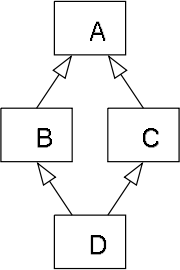
\includegraphics[scale=1.7]{informatika/programovanie/obrazky/diamond_inheritance.png}
      \caption{Diamond problem}
    \end{center}
  \end{figure}
\\\\  
\textbf{Implementace probl�mu Diamant v C++:} Postupuje po obou cest�ch odd�len�, tak�e objekt D pak obsahuje
2 separ�tn� A objekty a k�d pravd�podobn� skon�� na COMPILE ERROR. Pokud je d�di�nost z A do B a A do C ozna�ena jako "virtual" (nap��klad
"class B : virtual public A"), C++ pak vytvo�� pouze 1  A objekt a jeho ��sti
budou spr�vn� fungovat. Pokud ale sm�ch�me na obou
virtu�ln� a nevirtu�ln� d�di�nost dojde tak� ke COMPILE ERROR - p�i p��stupu
k ��stem A z D. 

 
\end{obecne}
\begin{obecne}{Virtu�ln� metody}
V objektov� orientovan�m programov�n� se pod pojmem virtu�ln� funkce nebo virtu�ln� metoda mysl� funkce/metoda (v k�du ozna�en� kl��ov�m slovem � typicky virtual), jej� chov�n� je ur�eno definic� v posledn�m objektu (ve sm�ru d�di�nosti od rodi�� k potomk�m), kter� definici funkce s danou signaturou obsahuje. Tento koncept je d�le�itou sou��st� polymorfismu v objektov� orientovan�m programov�n�.
\\\\Koncept virtu�ln�ch funkc� �e�� n�sleduj�c� probl�m:

Kdy� v OOP d�d� n�jak� t��da od jin�, tak instance pod�d�n� t��dy m��e b�t p�etypov�na na libovoln�ho ze sv�ch p�edk�. Pokud v�ak pod�d�n� t��da p�edefinovala pod�d�nou metody, nebude p�i jej�m p�etypov�n� na p�edka jasn�, kterou z definic� metody pou��t.
\\\\
Rozhodnut� ot�zky, kterou funkci zavolat, p�in�� pr�v� rozd�len� metod na virtu�ln� a nevirtu�ln�. Kdy� je funkce ozna�ena jako virtu�ln�, je pou�ita definice funkce z pod�d�n� t��dy (pokud existuje). V opa�n�m p��pad� je pou�ita definice ze t��dy na kterou je instance t��dy pr�v� p�etypov�na.
\\\\
\emph{Pozdn� vazba (late binding; virtual call):} Je-li metoda n�jak� t��dy virtu�ln� �i �ist� virtu�ln�, pak v�echny metody se stejn�m jm�nem, po�tem a typy parametr� deklarovan� v potomc�ch t��dy jsou pova�ov�ny za r�zn� implementace t�e funkce. Kter� implementace se vybere, tedy kter� t�lo bude zavol�no, se rozhoduje a� za b�hu programu podle skute�n�ho typu cel�ho objektu. Pou�ije se t�lo z posledn�ho potomka, kter� definuje tuto funkci a je sou��st� cel�ho objektu. Pozdn� vazba m� smysl pouze u vyvol�n� na objektu ur�en�m odkazem.

Pozdn� vazba je implementa�n� umo�n�n� skryt�m pointerem na \emph{tabulku virtu�ln�ch funkc� (VMT)} uvnit� ka�d�ho objektu. Existuje pro ka�dou t��du jedna. P�i d�di�nosti z�st�v� v cel�m objektu odkaz jeden (v C++ jich m��e
b�t p�i v�sen�sobn� d�di�nosti i v�ce), ale (i pro \uv{nejvnit�n�j��} b�zovou t��du) odkazuje na tabulku odvozen� t��dy. V tabulce mus� b�t proto pointery na funkce, deklarovan� u� u b�zov� t��dy, um�st�ny na za��tku (aby bylo mo�n� volat funkce b�zov� t��dy mezi sebou bez zm�ny k�du).
\end{obecne}



\begin{obecne}{Polymorfismus}Odkazovan� objekt se chov� podle toho, jak� je jeho skute�n� typ. Pokud n�kolik objekt� poskytuje stejn� rozhran�, pracuje se s nimi stejn�m zp�sobem, ale jejich konkr�tn� chov�n� se li��. V praxi se tato vlastnost projevuje nap�. tak, �e na m�sto, kde je o�ek�v�na instance n�jak� t��dy, m��eme dosadit i instanci libovoln� jej� podt��dy (t��dy, kter� p��mo �i nep��mo z t�to t��dy d�d�), kter� se m��e chovat jinak, ne� by se chovala instance rodi�ovsk� t��dy, ov�em v r�mci \uv{mantinel�}, dan�ch popisem rozhran�.
\end{obecne}
\newpage
\begin{obecne}{P��klad polymorfismu, d�di�nosti (p��padn� zapouzd�en�) v C\#:}
\begin{footnotesize}
\begin{verbatim}
namespace Program
{
    public interface IAnimal
    {
        string Name { get; }
        string Talk();
    }
    
    public abstract class AnimalBase
    {
        public string Name { get; private set; }
 
        protected AnimalBase(string name) {
            Name = name;
        }
    }
 
    public class Cat : AnimalBase, IAnimal
    {
        public Cat(string name) : base(name) {
        }
 
        public string Talk() {
            return "Meowww!";
        }
    }
 
    public class Dog : AnimalBase, IAnimal
    {
        public Dog(string name) : base(name) {            
        }
 
        public string Talk() {
            return "Arf! Arf!";
        }
    }
    
    public class TestAnimals
    {
        // prints the following:
        //   Missy: Meowww!
        //   Mr. Mistoffelees: Meowww!
        //   Lassie: Arf! Arf!
        //
        public static void Main(string[] args)
        {
            var animals = new List<IAnimal>() {
                new Cat("Missy"),
                new Cat("Mr. Mistoffelees"),
                new Dog("Lassie")
            };
 
            foreach (var animal in animals) {
                Console.WriteLine(animal.Name + ": " + animal.Talk());
            }
        }
    }
}
\end{verbatim}
\end{footnotesize}
\end{obecne}


\subsection{Neprocedurální programování, logické programování}

\subsubsection*{Neprocedurální programování}
\emph{Deklarativní programování} je postaveno na paradigmatu, podle něhož je program založen na tom, co se počítá a ne jak se to počítá. Je zde deklarován vstup a výstup a celý program je chápán jako funkce vyhodnocující vstupy podávající jediný výstup. Například i webovské stránky jsou deklarativní protože popisují, jak by stránka měla vypadat -- titulek, font, text a obrázky -- ale nepopisují, jak konkrétně zobrazit stránky na obrazovce.

\emph{Logické programování} a \emph{funkcionální programování} jsou poddruhy deklarativního programování. Logické programování využívá programování založené na vyhodnocování vzorů - tvrzení a cílů. Klasickým zástupcem jazyka pro podporu tohoto stylu je Prolog.

Tento přístup patří pod deklarativní programování stejně jako funkcionální programování, neboť deklaruje, co je vstupem a co výstupem, a nezabývá se jak výpočet probíhá. Naopak program jako posloupnost příkazů je paradigma imperativní.

\emph{Funkcionální programování} patří mezi deklarativní programovací principy.

Alonzo Church vytvořil formální výpočtový model nazvaný $\lambda$-kalkul. Tento model slouží jako základ pro funkcionální jazyky. Funkcionální jazyky dělíme na:
\begin{pitemize}
	\item typované - Haskell
	\item netypované - Lisp, Scheme
\end{pitemize}

Výpočtem funkcionálního programu je posloupnost vzájemně ekvivalentních výrazů, které se postupně zjednodušují. Výsledkem výpočtu je výraz v normální formě, tedy dále nezjednodušitelný. Program je chápán jako jedna funkce obsahující vstupní parametry mající jediný výstup. Tato funkce pak může být dále rozložitelná na podfunkce.

\subsubsection*{Prolog}

Prolog je logický programovací jazyk. Název Prolog pochází z francouzského programmation en logique (\uv{logické programování}). Byl vytvořen Alainem Colmerauerem v roce 1972 jako pokus vytvořit programovací jazyk, který by umožňoval vyjadřování v logice místo psaní počítačových instrukcí. Prolog patří mezi tzv. deklarativní programovací jazyky, ve kterých programátor popisuje pouze cíl výpočtu, přičemž přesný postup, jakým se k výsledku program dostane, je ponechán na libovůli systému.

Prolog je využíván především v oboru umělé inteligence a v počítačové lingvistice (obzvláště zpracování přirozeného jazyka, pro nějž byl původně navržen). Syntaxe jazyka je velice jednoduchá a snadno použitelná pravě proto, že byl původně určen pro počítačově nepříliš gramotné lingvisty.

Prolog je založen na \emph{predikátové logice prvního řádu} (konkrétně se omezuje na Hornovy klauzule). Běh programu je pak představován aplikací dokazovacích technik na zadané klauzule. Základními využívanými přístupy jsou \emph{unifikace}, \emph{rekurze} a \emph{backtracking}.

Interpret Prologu se snaží nalézt nejobecnější substituci, která splní daný cíl - tzn. nesubstituuje zbytečně, pokud nemusí (použití interních proměnných -- \_123 atd.). Za dvě proměnné může být substituována jedna interní proměnná (např. při hledání svislé úsečky -- konstantní X souřadnice) -- tomu se říká \emph{unifikace} proměnných. Pro proměnnou, jejíž hodnota může být libovolná, se v prologu užívá znak \uv{\_}. 

Datové typy v prologu se nazývají \emph{termy}. Základním datovým typem jsou \emph{atomy} (začínají malým písmenem, nebo se skládají ze speciálních znaků (\texttt{+ - * / \dots}, nebo jsou to znakové řetězce (\texttt{'text'})). Dále \uv{jsou} v prologu čísla (v komerčních implementacích i reálná), proměnné (velké písmeno) a struktury (definované rekursivně - pomocí funktoru dané arity a příslušným počtem termů, které jsou jeho argumenty -- \texttt{okamzik(datum(1,1,1999),cas(10,10))}). Posledním typem proměnných jsou seznamy, které jsou probírány později.

\medskip\textbf{Základní principy}:

Programování v Prologu se výrazně liší od programování v běžných procedurálních jazycích jako např. C. Program v prologu je databáze faktů a pravidel (dohromady se faktům a pravidlům paradoxně říká procedury), nad kterými je možno klást dotazy formou tvrzení, u kterých Prolog zhodnocuje jejich pravdivost (dokazatelnost z údajů obsažených v databázi).

Například lze do databáze uložit fakt, že Monika je dívka:
\begin{verbatim}
dívka(monika).
\end{verbatim}

Poté lze dokazatelnost tohoto faktu prověřit otázkou, na kterou Prolog odpoví yes (ano):
\begin{verbatim}
?- dívka(monika).
     yes.
\end{verbatim}

Také se lze zeptat na všechny objekty, o kterých je známo, že jsou dívky (středníkem požadujeme další výsledky):
\begin{verbatim}
?- dívka(X).
     X = monika;
     no.
\end{verbatim}

Pravidla (závislosti) se zapisují pomocí implikací, např.
\begin{verbatim}
syn(A,B) :- rodič(B,A), muž(A).
\end{verbatim}

Tedy: pokud B je rodičem A a zároveň je A muž, pak A je synem B. První části pravidla (tj. důsledku) se říká hlava a všemu co následuje za symbolem \texttt{:-} (tedy podmínkám, nutným pro splnění hlavy) se říká tělo. Podmínky ke splnění mohou být odděleny buď čárkou (pak jde o konjunkci, musejí být splněny všechny), nebo středníkem (disjunkce), přičemž čárky mají větší prioritu.

\medskip\textbf{Příklad}:

Typickou ukázkou základů programování v Prologu jsou rodinné vztahy.
\begin{verbatim}
sourozenec(X,Y) :- rodič(Z,X), rodič(Z,Y).
rodič(X,Y) :- otec(X,Y).
rodič(X,Y) :- matka(X,Y).
muž(X) :- otec(X,_).
žena(X) :- matka(X,_).
matka(marie,monika).
otec(jiří,monika).
otec(jiří,marek).
otec(michal,tomáš).
\end{verbatim}

Prázdný seznam je označen atomem $[]$, neprázdný se tvoří pomocí funktoru \texttt{'.'} (tečka) - \texttt{.(Hlava,Tělo)}. V praxi se to (naštěstí ;-)) takhle složitě rekurzivně zapisovat nemusí, stačí napsat \texttt{[a,b,c...]}, resp \texttt{[Začátek | Tělo]}, kde začátek je výčet prvků (ne seznam) stojících na začátku definovaného seznamu, a tělo je (rekurzivně) seznam (např. \texttt{[a,b,c|[]]}).

Aritmetické výrazy se samy o sobě nevyhodnocují, dokud jim to někdo nepřikáže. Takže např. predikát \texttt{5*1 = 5} by selhal. Vyhodnocení se vynucuje pomocí operátoru \emph{is} (pomocí = by došlo jen k unifikaci) - není to ale ekvivalent \uv{\texttt{=}} z jiných jazyků. Tento operátor se musí použít na nějakou volnou proměnnou a aritmetický výraz, s jehož hodnotou bude tato proměnná dále svázaná (jako např. \texttt{X is 5*1,X=5} uspěje).

Důležitý je i \emph{operátor řezu} (značíme vykřičníkem). Tento predikát okamžitě uspěje, ale při tom zakáže backtrackování přes sebe zpět. (\texttt{prvek1(X,[X|L]):-!. prvek1(X,[\_|L]):-prvek1(X,L).} - je-li prvek nalezen, je zakázán návrat = najde jen první výskyt prvku). Dále je důležitá negace (\texttt{not(P):- P, !, fail. not(P).} -- uspěje, pokud se nepodaří cíl P splnit). Řez tedy umožňuje ovlivňovat efektivitu prologovských programů, definovat vzájemně se vylučující použití jednotlivých klauzulí procedury, definovat negaci atd.

\subsubsection*{Haskell}
Haskell je standardizovaný funkcionální programovací jazyk používající zkrácené vyhodnocování, pojmenovaný na počest logika Haskella Curryho. Byl vytvořen v 80. letech 20. století. Posledním polooficiálním standardem je Haskell 98, který definuje minimální a přenositelnou verzi jazyka využitelnou k výuce nebo jako základ dalších rozšíření. Jazyk se rychle vyvíjí, především díky svým implementacím Hugs a GHC (viz níže).

Haskell je jazyk dodržující \emph{referenční transparentnost}. To, zjednodušeně řečeno, znamená, že tentýž (pod)výraz má na jakémkoliv místě v programu stejnou hodnotu. Mezi další výhody tohoto jazyka patří přísné \emph{typování proměnných}, které programátorovi může usnadnit odhalování chyb v programu. Haskell plně podporuje práci se soubory i standardními vstupy a výstupy, která je ale poměrně složitá kvůli zachování referenční transparentnosti. Jako takový se Haskell hodí hlavně pro algoritmicky náročné úlohy minimalizující interakci s uživatelem.

\medskip\textbf{Příklady}:

Definice funkce faktoriálu:
\begin{verbatim}
fac 0 = 1
fac n = n * fac (n - 1)
\end{verbatim}

Jiná definice faktoriálu (používá funkci product ze standardní knihovny Haskellu):
\begin{verbatim}
fac n = product [1..n]
\end{verbatim}

Naivní implementace funkce vracející n-tý prvek Fibonacciho posloupnosti:
\begin{verbatim}
fib 0 = 0 
fib 1 = 1 
fib n = fib (n - 2) + fib (n - 1)
\end{verbatim}

Elegantní zápis řadícího algoritmu quicksort:
\begin{verbatim}
qsort [] = []
qsort (pivot:tail) = 
  qsort left ++ [pivot] ++ qsort right
  where
    left = [y | y <- tail, y < pivot]
    right = [y | y <- tail, y >= pivot]
\end{verbatim}

TODO: popsat stráže (případy, otherwise), seznamy, řetězení, pattern matching u parametrů funkcí, lok. definice (where, let) -- patří to sem?

\subsubsection*{Lisp}

Lisp je funkcionální programovací jazyk s dlouhou historií. Jeho název je zkratka pro List processing (zpracování seznamů). Dnes se stále používá v oboru umělé inteligence. Nic ale nebrání ho použít i pro jiné účely. Používá ho například textový editor Emacs, GIMP či konstrukční program AutoCAD.

Další jazyky od něj odvozené jsou například Tcl, Smalltalk nebo Scheme.


\medskip\textbf{Syntaxe}:
Nejzákladnějším zápisem v Lispu je seznam. Zapisujeme ho jako:
\begin{verbatim}
(1 2 "ahoj" 13.2)
\end{verbatim}

Tento seznam obsahuje čtyři prvky:
\begin{pitemize}
	\item celé číslo 1
	\item celé číslo 2
	\item text \uv{ahoj}
	\item reálné číslo 13,2
\end{pitemize}

Jde tedy o uspořádanou čtveřici. Všimněte si, že závorky nefungují tak jako v matematice, ale pouze označují začátek a konec seznamu. Seznamy jsou v Lispu implementovány jako binární strom degenerovaný na jednosměrně vázaný seznam. Co se seznamem Lisp udělá, záleží na okolnostech.

\textbf{Příkazy}: Příkazy píšeme také jako seznam, první prvek seznamu je však název příkazu. Například sčítání provádíme příkazem +, což interpreteru zadáme takto:
\begin{verbatim}
(+ 1 2 3)
\end{verbatim}
Interpretr odpoví 6.

\textbf{Ukázka kódu}:
Program hello world lze zapsat několika způsoby. Nejjednoduší vypadá takto:
\begin{verbatim}
(format t "Hello, World!")
\end{verbatim}

Funkce se v Lispu definují pomocí klíčového slova defun:
\begin{verbatim}
(defun hello ()
        (format t "Hello, World!")
)
(hello)
\end{verbatim}

Na prvních dvou řádcích je definice funkce hello, na třetím řádku je tato funkce svým jménem zavolána.
Funkcím lze předávat i argumenty. V následujícím příkladu je ukázka funkce fact, která vypočítá faktoriál zadaného čísla:
\begin{verbatim}
(defun fact (n)
        (if (= n 0)
                1
                (* n (fact (- n 1)))
        )
)
\end{verbatim}
Pro výpočet faktoriálu čísla 6 předáme tuto hodnotu jako argument funkci fact:
\begin{verbatim}
(fact 6)
\end{verbatim}
Návratovou hodnotou funkce bude hodnota 720.

\subsubsection*{Logické programování}
TODO (není součástí otázek pro obor Programování)

\subsection{Generick� programov�n� � �ablony a generika}

Z�kladn� my�lenkou, kter� se skr�v� za pojmem generick� programov�n�, je rozd�len� k�du programu na algoritmus a datov� typy takov�m zp�sobem, aby bylo mo�n� z�pis k�du algoritmu ch�pat jako obecn�, bez ohledu na to, nad jak�mi datov�mi typy pracuje. Konkr�tn� k�d algoritmu se z n�j st�v� dosazen�m datov�ho typu.

U kompilovan�ch jazyk� doch�z� k rozvinut� k�du v dob� p�ekladu. Typick�m p��kladem jazyka, kter� podporuje tuto formu generick�ho programov�n�, je jazyk C++. Mechanismem, kter� zde generick� programov�n� umo��uje, 
jsou takzvan� �ablony (templates).

\medskip
\begin{poznamkaN}{Metaprogramov�n� a Generika}
It differs from normal programming in that it somehow invokes within the language a metaprogramming facility. Because it happens as an extension of the language, new semantics are introduced and the language is enriched in this process. It is closely related to metaprogramming, but does not involve the generation of source code (none, at least, that is visible to the user of the language). It is different from programming with macros as well, as the latter refers to textual search-and-replace and is not part of the grammar of the language but implemented by a pre-processor. One exception to this is the macro facility in Common Lisp, in which macros operate on parse trees rather than text.

Oby�ejn� fce maj� p�ednost p�ed generick�mi???
\end{poznamkaN}

\begin{definiceN}{�ablony}
Template metaprogramming is a metaprogramming technique in which templates are used by a compiler to generate temporary source code, which is merged by the compiler with the rest of the source code and then compiled. The output of these templates include compile-time constants, data structures, and complete functions. The use of templates can be thought of as compile-time execution. The technique is used by a number of languages, the best-known being C++, but also Curl, D, and XL.
\end{definiceN}

\begin{prikladN}{T��da parametrizovan� typem (kontejner)}
As an example of the benefits of generic programming, when creating containers of objects it is common to write specific implementations for each datatype contained, even if the code is virtually identical except for different datatypes. Instead, a possible declaration using generic programming could be to define a template class (using the C++ idiom):
\begin{verbatim}
  template<typename T> 
  class List 
  { 
    T x;
    List<T> *next;
  };
  
  List<Animal> list_of_animals;
  List<Car> list_of_cars;
  
  ...
  
  conductor = root;
  while ( conductor != NULL ) {
    cout<< conductor->x;
    conductor = conductor->next;
  }
\end{verbatim}
Above T represents the type to be instantiated. The list generated is then treated as a list of whichever type is specified. These "containers-of-type-T", commonly called generics, are a generic programming technique that allows the defining of a class that takes and contains different datatypes (not to be confused with polymorphism, which is the algorithmic usage of exchangeable sub-classes) as long as certain contracts such as subtypes and signature are kept. Although the example above is the most common use of generic programming, and some languages implement only this aspect of it, generic programming as a concept is not limited to generics. 
\end{prikladN}

\begin{prikladN}{Typov� nez�visl� funkce}
Another applicaton is type-independent functions as in the Swap example below:
\begin{verbatim}
  template<typename T>
  void Swap(T & a, T & b) //"&" passes parameters by reference
  {
     T temp = b;
     b = a;
     a = temp;
  }
  
  string hello = "world!", world = "Hello, ";
  Swap( world, hello );
  cout << hello << world << endl; //Output is "Hello, world!"
\end{verbatim}
\end{prikladN}

\begin{prikladN}{Faktori�l pomoc� �ablon}
\begin{verbatim}
  template <int N>
  struct Factorial 
  {
      enum { value = N * Factorial<N - 1>::value };
  };
   
  template <>
  struct Factorial<0> 
  {
      enum { value = 1 };
  };
   
  // pou�it�:
  int x = Factorial<4>::value; // == 24
  int y = Factorial<0>::value; // == 1
\end{verbatim}
\end{prikladN}


\begin{prikladN}{traits}
Programovac� paradigma vyu��vaj�c� �ablony, ze kter�ch nejsou vytv��eny objekty. Ur�eny k dopln�n� informac� o n�jak�m typu.
\\\\Obsahuj� pouze:
\begin{pitemize}
\item Definice typ�
\item Statick� funkce
\end{pitemize}

\begin{verbatim}
  template< typename T > 
  struct is_void{ 
    static const bool value = false;
  };
  
  template<> 
  struct is_void< void >{ 
    static const bool value = true; 
  };
  
  // pou�it�:
  is_void<int>::value; // false
  is_void<void>::value; // true
\end{verbatim}
\end{prikladN}
\newpage
\begin{prikladN}{policy classes}
Ur�eny k definov�n� ur�it�ho chov�n�. Jous to t��dy, ze kter�ch obvykle nejsou vytv��eny objekty a jsou p�ed�v�ny jako parametr �ablon�m. Defaultn� hodnotou parametru �asto b�v� �ablona traits. Hlavn� spojen� s C++ (v ostatn�ch jazyc�ch se zat�m neroz���ilo).
\begin{verbatim}
  template < typename output_policy, typename language_policy >
  class HelloWorld : public output_policy, public language_policy
  {
      using output_policy::Print;
      using language_policy::Message;
       
      public: void Run() //behaviour method
      {
          //two policy methods
          Print( Message() );
      }
  };
   
  class OutputPolicy_WriteToCout
  {
   protected:
      template< typename message_type >
      void Print( message_type message )
      {
          std::cout << message << std::endl;
      }
  };
   
  class LanguagePolicy_English
  {
      protected: std::string Message() { return "Hello, World!"; }
  };
   
  class LanguagePolicy_German
  {
      protected: std::string Message() { return "Hallo Welt!"; }
  };
   
  int main()
  {
      /* example 1 */
      HelloWorld<OutputPolicy_WriteToCout, LanguagePolicy_English>  hello_world;
      hello_world.Run(); // Prints "Hello, World!"
   
     /* example 2 
      * does the same but uses another policy, the language has changed
      */
      HelloWorld<OutputPolicy_WriteToCout, LanguagePolicy_German> hello_world2;
      hello_world2.Run(); // Prints "Hallo Welt!"
  }
\end{verbatim}
\end{prikladN}
\newpage
\begin{definiceN}{Dynamick� (run-time) polymorfismus}
D�d�n� + VMT = flexibilita.
P��padn� jeho varianta s �ablonami:
\begin{verbatim}
class Base
{
public:
    virtual void method() { std::cout << "Base"; }
    virtual ~Base() {}
};
 
class Derived : public Base
{
public:
    virtual void method() { std::cout << "Derived"; }
};
 
int main()
{
    Base *pBase = new Derived;
    pBase->method(); //outputs "Derived"
    delete pBase;
    return 0;
}
\end{verbatim}
\end{definiceN}

\begin{definiceN}{Statick� (compile-time) polymorfismus}
Je p�et�ov�n� fukc� a oper�tor�, �e�� se p�i kompilaci = rychlost.
P��padn� jeho varianta s �ablonami:
\begin{verbatim}
template <class Derived>
struct base
{
    void interface()
    {
         // ...
         static_cast<Derived*>(this)->implementation();
         // ...
    }
};
 
struct derived : base<derived>
{
     void implementation();
};
\end{verbatim}
Lze tak dos�hnout podobn�ch v�c� jako s VMT.
\end{definiceN}

\begin{obecne}{Pou�it� v programovac�ch jazyc�ch}
The template construct of C++ used in the examples above is widely cited as the generic programming construct that popularized the notion among programmers and language designers and provides full support for all generic programming idioms. D also offers fully generic-capable templates based on the C++ precedent but with a simplified syntax. Java has provided generic programming facilities syntactically based on C++'s since the introduction of J2SE 5.0 and implements the generics, or "containers-of-type-T", subset of generic programming.
\end{obecne}

\begin{reportN}{IP 21.6.2011} Co je to generick� programov�n�, k �emu se pou��v� a v �em spo��vaj� jeho v�hody?

Napi�te stru�nou implementaci generick� t��dy List nebo HashTable.

Popi�te implementaci v C++ a Jav� (asi by sta�il i C#, ale v zad�n� byla explicitn� napsan� java).
\end{reportN}

\begin{reportN}{IP 21.6.2011 ($<$2007)} Popiste sablony
\\Jak jsou implementovany (popiste jak jsou implementovany v C++ nebo Java) (to som teda fakt netusil)
\end{reportN}

\begin{reportN}{IOI 21.6.2011 ($<$2007)}
Co je to generick� programov�n�, k �emu se pou��v� a v �em spo��vaj� jeho v�hody?

Napi�te stru�nou implementaci generick� t��dy List nebo HashTable.
\end{reportN}

\begin{reportN}{Yaghob}
Co je to traits a policy classes, co je to statick� polymorfismus apod. Nakonec jsem to n�jak vymyslel a shodli jsme se na tom, �e to v�m, tak�e taky za 1.
\end{reportN}


\end{document}
